% Created by tikzDevice version 0.12.6 on 2025-01-17 13:26:28
% !TEX encoding = UTF-8 Unicode
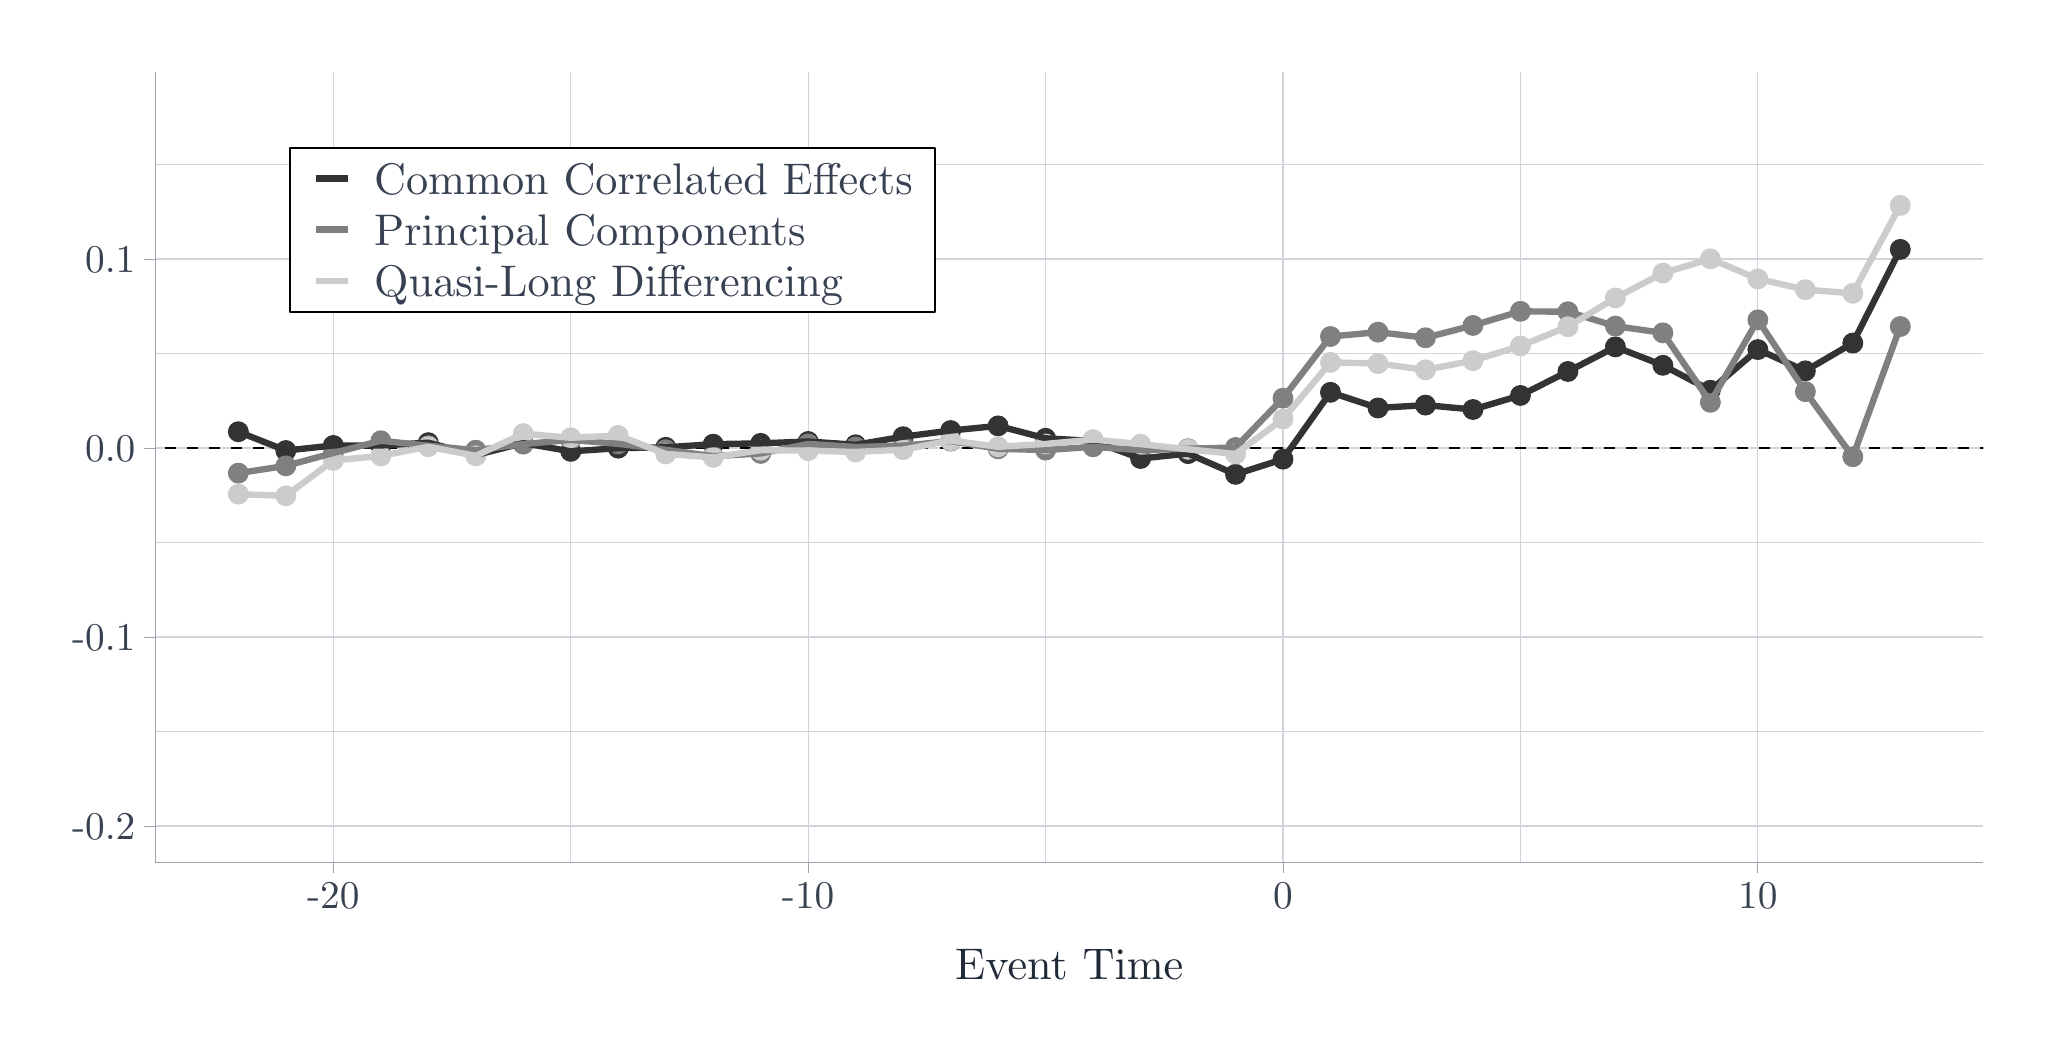
\begin{tikzpicture}[x=1pt,y=1pt]
\definecolor{fillColor}{RGB}{255,255,255}
\path[use as bounding box,fill=fillColor] (0,0) rectangle (722.70,361.35);
\begin{scope}
\path[clip] (  0.00,  0.00) rectangle (722.70,361.35);
\definecolor{drawColor}{RGB}{255,255,255}

\path[draw=drawColor,line width= 0.8pt,line join=round,line cap=round,fill=fillColor] (  0.00,  0.00) rectangle (722.70,361.35);
\end{scope}
\begin{scope}
\path[clip] ( 46.10, 59.89) rectangle (706.70,345.35);
\definecolor{drawColor}{RGB}{255,255,255}
\definecolor{fillColor}{RGB}{255,255,255}

\path[draw=drawColor,line width= 0.8pt,line join=round,line cap=round,fill=fillColor] ( 46.10, 59.89) rectangle (706.70,345.35);
\definecolor{drawColor}{RGB}{209,213,219}

\path[draw=drawColor,line width= 0.4pt,line join=round] ( 46.10,107.01) --
	(706.70,107.01);

\path[draw=drawColor,line width= 0.4pt,line join=round] ( 46.10,175.30) --
	(706.70,175.30);

\path[draw=drawColor,line width= 0.4pt,line join=round] ( 46.10,243.59) --
	(706.70,243.59);

\path[draw=drawColor,line width= 0.4pt,line join=round] ( 46.10,311.89) --
	(706.70,311.89);

\path[draw=drawColor,line width= 0.4pt,line join=round] (196.24, 59.89) --
	(196.24,345.35);

\path[draw=drawColor,line width= 0.4pt,line join=round] (367.82, 59.89) --
	(367.82,345.35);

\path[draw=drawColor,line width= 0.4pt,line join=round] (539.41, 59.89) --
	(539.41,345.35);

\path[draw=drawColor,line width= 0.4pt,line join=round] ( 46.10, 72.86) --
	(706.70, 72.86);

\path[draw=drawColor,line width= 0.4pt,line join=round] ( 46.10,141.16) --
	(706.70,141.16);

\path[draw=drawColor,line width= 0.4pt,line join=round] ( 46.10,209.45) --
	(706.70,209.45);

\path[draw=drawColor,line width= 0.4pt,line join=round] ( 46.10,277.74) --
	(706.70,277.74);

\path[draw=drawColor,line width= 0.4pt,line join=round] (110.45, 59.89) --
	(110.45,345.35);

\path[draw=drawColor,line width= 0.4pt,line join=round] (282.03, 59.89) --
	(282.03,345.35);

\path[draw=drawColor,line width= 0.4pt,line join=round] (453.61, 59.89) --
	(453.61,345.35);

\path[draw=drawColor,line width= 0.4pt,line join=round] (625.20, 59.89) --
	(625.20,345.35);
\definecolor{drawColor}{RGB}{0,0,0}

\path[draw=drawColor,line width= 0.9pt,dash pattern=on 4pt off 4pt ,line join=round] (-614.49,209.45) -- (1367.30,209.45);
\definecolor{drawColor}{gray}{0.20}
\definecolor{fillColor}{gray}{0.20}

\path[draw=drawColor,line width= 0.4pt,line join=round,line cap=round,fill=fillColor] ( 76.13,215.34) circle (  3.57);

\path[draw=drawColor,line width= 0.4pt,line join=round,line cap=round,fill=fillColor] ( 93.29,208.54) circle (  3.57);

\path[draw=drawColor,line width= 0.4pt,line join=round,line cap=round,fill=fillColor] (110.45,210.38) circle (  3.57);

\path[draw=drawColor,line width= 0.4pt,line join=round,line cap=round,fill=fillColor] (127.61,210.38) circle (  3.57);

\path[draw=drawColor,line width= 0.4pt,line join=round,line cap=round,fill=fillColor] (144.76,211.39) circle (  3.57);

\path[draw=drawColor,line width= 0.4pt,line join=round,line cap=round,fill=fillColor] (161.92,206.90) circle (  3.57);

\path[draw=drawColor,line width= 0.4pt,line join=round,line cap=round,fill=fillColor] (179.08,211.23) circle (  3.57);

\path[draw=drawColor,line width= 0.4pt,line join=round,line cap=round,fill=fillColor] (196.24,208.24) circle (  3.57);

\path[draw=drawColor,line width= 0.4pt,line join=round,line cap=round,fill=fillColor] (213.40,209.40) circle (  3.57);

\path[draw=drawColor,line width= 0.4pt,line join=round,line cap=round,fill=fillColor] (230.56,209.71) circle (  3.57);

\path[draw=drawColor,line width= 0.4pt,line join=round,line cap=round,fill=fillColor] (247.71,210.85) circle (  3.57);

\path[draw=drawColor,line width= 0.4pt,line join=round,line cap=round,fill=fillColor] (264.87,211.14) circle (  3.57);

\path[draw=drawColor,line width= 0.4pt,line join=round,line cap=round,fill=fillColor] (282.03,211.82) circle (  3.57);

\path[draw=drawColor,line width= 0.4pt,line join=round,line cap=round,fill=fillColor] (299.19,210.63) circle (  3.57);

\path[draw=drawColor,line width= 0.4pt,line join=round,line cap=round,fill=fillColor] (316.35,213.55) circle (  3.57);

\path[draw=drawColor,line width= 0.4pt,line join=round,line cap=round,fill=fillColor] (333.51,215.77) circle (  3.57);

\path[draw=drawColor,line width= 0.4pt,line join=round,line cap=round,fill=fillColor] (350.66,217.45) circle (  3.57);

\path[draw=drawColor,line width= 0.4pt,line join=round,line cap=round,fill=fillColor] (367.82,212.97) circle (  3.57);

\path[draw=drawColor,line width= 0.4pt,line join=round,line cap=round,fill=fillColor] (384.98,212.01) circle (  3.57);

\path[draw=drawColor,line width= 0.4pt,line join=round,line cap=round,fill=fillColor] (402.14,205.66) circle (  3.57);

\path[draw=drawColor,line width= 0.4pt,line join=round,line cap=round,fill=fillColor] (419.30,207.43) circle (  3.57);

\path[draw=drawColor,line width= 0.4pt,line join=round,line cap=round,fill=fillColor] (436.46,199.94) circle (  3.57);

\path[draw=drawColor,line width= 0.4pt,line join=round,line cap=round,fill=fillColor] (453.61,205.43) circle (  3.57);

\path[draw=drawColor,line width= 0.4pt,line join=round,line cap=round,fill=fillColor] (470.77,229.58) circle (  3.57);

\path[draw=drawColor,line width= 0.4pt,line join=round,line cap=round,fill=fillColor] (487.93,223.93) circle (  3.57);

\path[draw=drawColor,line width= 0.4pt,line join=round,line cap=round,fill=fillColor] (505.09,224.96) circle (  3.57);

\path[draw=drawColor,line width= 0.4pt,line join=round,line cap=round,fill=fillColor] (522.25,223.37) circle (  3.57);

\path[draw=drawColor,line width= 0.4pt,line join=round,line cap=round,fill=fillColor] (539.41,228.45) circle (  3.57);

\path[draw=drawColor,line width= 0.4pt,line join=round,line cap=round,fill=fillColor] (556.56,237.11) circle (  3.57);

\path[draw=drawColor,line width= 0.4pt,line join=round,line cap=round,fill=fillColor] (573.72,246.00) circle (  3.57);

\path[draw=drawColor,line width= 0.4pt,line join=round,line cap=round,fill=fillColor] (590.88,239.34) circle (  3.57);

\path[draw=drawColor,line width= 0.4pt,line join=round,line cap=round,fill=fillColor] (608.04,230.34) circle (  3.57);

\path[draw=drawColor,line width= 0.4pt,line join=round,line cap=round,fill=fillColor] (625.20,245.03) circle (  3.57);

\path[draw=drawColor,line width= 0.4pt,line join=round,line cap=round,fill=fillColor] (642.36,237.34) circle (  3.57);

\path[draw=drawColor,line width= 0.4pt,line join=round,line cap=round,fill=fillColor] (659.51,247.38) circle (  3.57);

\path[draw=drawColor,line width= 0.4pt,line join=round,line cap=round,fill=fillColor] (676.67,281.23) circle (  3.57);
\definecolor{drawColor}{gray}{0.50}
\definecolor{fillColor}{gray}{0.50}

\path[draw=drawColor,line width= 0.4pt,line join=round,line cap=round,fill=fillColor] ( 76.13,200.38) circle (  3.57);

\path[draw=drawColor,line width= 0.4pt,line join=round,line cap=round,fill=fillColor] ( 93.29,203.01) circle (  3.57);

\path[draw=drawColor,line width= 0.4pt,line join=round,line cap=round,fill=fillColor] (110.45,207.65) circle (  3.57);

\path[draw=drawColor,line width= 0.4pt,line join=round,line cap=round,fill=fillColor] (127.61,212.08) circle (  3.57);

\path[draw=drawColor,line width= 0.4pt,line join=round,line cap=round,fill=fillColor] (144.76,210.30) circle (  3.57);

\path[draw=drawColor,line width= 0.4pt,line join=round,line cap=round,fill=fillColor] (161.92,208.67) circle (  3.57);

\path[draw=drawColor,line width= 0.4pt,line join=round,line cap=round,fill=fillColor] (179.08,210.87) circle (  3.57);

\path[draw=drawColor,line width= 0.4pt,line join=round,line cap=round,fill=fillColor] (196.24,212.38) circle (  3.57);

\path[draw=drawColor,line width= 0.4pt,line join=round,line cap=round,fill=fillColor] (213.40,210.97) circle (  3.57);

\path[draw=drawColor,line width= 0.4pt,line join=round,line cap=round,fill=fillColor] (230.56,208.82) circle (  3.57);

\path[draw=drawColor,line width= 0.4pt,line join=round,line cap=round,fill=fillColor] (247.71,206.49) circle (  3.57);

\path[draw=drawColor,line width= 0.4pt,line join=round,line cap=round,fill=fillColor] (264.87,207.50) circle (  3.57);

\path[draw=drawColor,line width= 0.4pt,line join=round,line cap=round,fill=fillColor] (282.03,210.93) circle (  3.57);

\path[draw=drawColor,line width= 0.4pt,line join=round,line cap=round,fill=fillColor] (299.19,209.81) circle (  3.57);

\path[draw=drawColor,line width= 0.4pt,line join=round,line cap=round,fill=fillColor] (316.35,210.31) circle (  3.57);

\path[draw=drawColor,line width= 0.4pt,line join=round,line cap=round,fill=fillColor] (333.51,211.95) circle (  3.57);

\path[draw=drawColor,line width= 0.4pt,line join=round,line cap=round,fill=fillColor] (350.66,209.17) circle (  3.57);

\path[draw=drawColor,line width= 0.4pt,line join=round,line cap=round,fill=fillColor] (367.82,208.71) circle (  3.57);

\path[draw=drawColor,line width= 0.4pt,line join=round,line cap=round,fill=fillColor] (384.98,209.89) circle (  3.57);

\path[draw=drawColor,line width= 0.4pt,line join=round,line cap=round,fill=fillColor] (402.14,208.67) circle (  3.57);

\path[draw=drawColor,line width= 0.4pt,line join=round,line cap=round,fill=fillColor] (419.30,209.21) circle (  3.57);

\path[draw=drawColor,line width= 0.4pt,line join=round,line cap=round,fill=fillColor] (436.46,209.65) circle (  3.57);

\path[draw=drawColor,line width= 0.4pt,line join=round,line cap=round,fill=fillColor] (453.61,227.46) circle (  3.57);

\path[draw=drawColor,line width= 0.4pt,line join=round,line cap=round,fill=fillColor] (470.77,249.75) circle (  3.57);

\path[draw=drawColor,line width= 0.4pt,line join=round,line cap=round,fill=fillColor] (487.93,251.33) circle (  3.57);

\path[draw=drawColor,line width= 0.4pt,line join=round,line cap=round,fill=fillColor] (505.09,249.29) circle (  3.57);

\path[draw=drawColor,line width= 0.4pt,line join=round,line cap=round,fill=fillColor] (522.25,253.75) circle (  3.57);

\path[draw=drawColor,line width= 0.4pt,line join=round,line cap=round,fill=fillColor] (539.41,258.85) circle (  3.57);

\path[draw=drawColor,line width= 0.4pt,line join=round,line cap=round,fill=fillColor] (556.56,258.69) circle (  3.57);

\path[draw=drawColor,line width= 0.4pt,line join=round,line cap=round,fill=fillColor] (573.72,253.51) circle (  3.57);

\path[draw=drawColor,line width= 0.4pt,line join=round,line cap=round,fill=fillColor] (590.88,251.06) circle (  3.57);

\path[draw=drawColor,line width= 0.4pt,line join=round,line cap=round,fill=fillColor] (608.04,225.97) circle (  3.57);

\path[draw=drawColor,line width= 0.4pt,line join=round,line cap=round,fill=fillColor] (625.20,255.76) circle (  3.57);

\path[draw=drawColor,line width= 0.4pt,line join=round,line cap=round,fill=fillColor] (642.36,229.83) circle (  3.57);

\path[draw=drawColor,line width= 0.4pt,line join=round,line cap=round,fill=fillColor] (659.51,206.31) circle (  3.57);

\path[draw=drawColor,line width= 0.4pt,line join=round,line cap=round,fill=fillColor] (676.67,253.36) circle (  3.57);
\definecolor{drawColor}{gray}{0.80}
\definecolor{fillColor}{gray}{0.80}

\path[draw=drawColor,line width= 0.4pt,line join=round,line cap=round,fill=fillColor] ( 76.13,192.80) circle (  3.57);

\path[draw=drawColor,line width= 0.4pt,line join=round,line cap=round,fill=fillColor] ( 93.29,192.17) circle (  3.57);

\path[draw=drawColor,line width= 0.4pt,line join=round,line cap=round,fill=fillColor] (110.45,204.98) circle (  3.57);

\path[draw=drawColor,line width= 0.4pt,line join=round,line cap=round,fill=fillColor] (127.61,206.58) circle (  3.57);

\path[draw=drawColor,line width= 0.4pt,line join=round,line cap=round,fill=fillColor] (144.76,209.94) circle (  3.57);

\path[draw=drawColor,line width= 0.4pt,line join=round,line cap=round,fill=fillColor] (161.92,206.63) circle (  3.57);

\path[draw=drawColor,line width= 0.4pt,line join=round,line cap=round,fill=fillColor] (179.08,214.65) circle (  3.57);

\path[draw=drawColor,line width= 0.4pt,line join=round,line cap=round,fill=fillColor] (196.24,213.15) circle (  3.57);

\path[draw=drawColor,line width= 0.4pt,line join=round,line cap=round,fill=fillColor] (213.40,214.01) circle (  3.57);

\path[draw=drawColor,line width= 0.4pt,line join=round,line cap=round,fill=fillColor] (230.56,207.32) circle (  3.57);

\path[draw=drawColor,line width= 0.4pt,line join=round,line cap=round,fill=fillColor] (247.71,206.05) circle (  3.57);

\path[draw=drawColor,line width= 0.4pt,line join=round,line cap=round,fill=fillColor] (264.87,208.66) circle (  3.57);

\path[draw=drawColor,line width= 0.4pt,line join=round,line cap=round,fill=fillColor] (282.03,208.51) circle (  3.57);

\path[draw=drawColor,line width= 0.4pt,line join=round,line cap=round,fill=fillColor] (299.19,208.03) circle (  3.57);

\path[draw=drawColor,line width= 0.4pt,line join=round,line cap=round,fill=fillColor] (316.35,208.87) circle (  3.57);

\path[draw=drawColor,line width= 0.4pt,line join=round,line cap=round,fill=fillColor] (333.51,212.16) circle (  3.57);

\path[draw=drawColor,line width= 0.4pt,line join=round,line cap=round,fill=fillColor] (350.66,209.90) circle (  3.57);

\path[draw=drawColor,line width= 0.4pt,line join=round,line cap=round,fill=fillColor] (367.82,210.93) circle (  3.57);

\path[draw=drawColor,line width= 0.4pt,line join=round,line cap=round,fill=fillColor] (384.98,212.51) circle (  3.57);

\path[draw=drawColor,line width= 0.4pt,line join=round,line cap=round,fill=fillColor] (402.14,210.86) circle (  3.57);

\path[draw=drawColor,line width= 0.4pt,line join=round,line cap=round,fill=fillColor] (419.30,209.00) circle (  3.57);

\path[draw=drawColor,line width= 0.4pt,line join=round,line cap=round,fill=fillColor] (436.46,207.29) circle (  3.57);

\path[draw=drawColor,line width= 0.4pt,line join=round,line cap=round,fill=fillColor] (453.61,219.94) circle (  3.57);

\path[draw=drawColor,line width= 0.4pt,line join=round,line cap=round,fill=fillColor] (470.77,240.40) circle (  3.57);

\path[draw=drawColor,line width= 0.4pt,line join=round,line cap=round,fill=fillColor] (487.93,239.97) circle (  3.57);

\path[draw=drawColor,line width= 0.4pt,line join=round,line cap=round,fill=fillColor] (505.09,237.72) circle (  3.57);

\path[draw=drawColor,line width= 0.4pt,line join=round,line cap=round,fill=fillColor] (522.25,241.03) circle (  3.57);

\path[draw=drawColor,line width= 0.4pt,line join=round,line cap=round,fill=fillColor] (539.41,246.35) circle (  3.57);

\path[draw=drawColor,line width= 0.4pt,line join=round,line cap=round,fill=fillColor] (556.56,253.30) circle (  3.57);

\path[draw=drawColor,line width= 0.4pt,line join=round,line cap=round,fill=fillColor] (573.72,263.69) circle (  3.57);

\path[draw=drawColor,line width= 0.4pt,line join=round,line cap=round,fill=fillColor] (590.88,272.67) circle (  3.57);

\path[draw=drawColor,line width= 0.4pt,line join=round,line cap=round,fill=fillColor] (608.04,277.81) circle (  3.57);

\path[draw=drawColor,line width= 0.4pt,line join=round,line cap=round,fill=fillColor] (625.20,270.56) circle (  3.57);

\path[draw=drawColor,line width= 0.4pt,line join=round,line cap=round,fill=fillColor] (642.36,266.67) circle (  3.57);

\path[draw=drawColor,line width= 0.4pt,line join=round,line cap=round,fill=fillColor] (659.51,265.36) circle (  3.57);

\path[draw=drawColor,line width= 0.4pt,line join=round,line cap=round,fill=fillColor] (676.67,297.13) circle (  3.57);
\definecolor{drawColor}{gray}{0.20}

\path[draw=drawColor,line width= 2.3pt,line join=round] ( 76.13,215.34) --
	( 93.29,208.54) --
	(110.45,210.38) --
	(127.61,210.38) --
	(144.76,211.39) --
	(161.92,206.90) --
	(179.08,211.23) --
	(196.24,208.24) --
	(213.40,209.40) --
	(230.56,209.71) --
	(247.71,210.85) --
	(264.87,211.14) --
	(282.03,211.82) --
	(299.19,210.63) --
	(316.35,213.55) --
	(333.51,215.77) --
	(350.66,217.45) --
	(367.82,212.97) --
	(384.98,212.01) --
	(402.14,205.66) --
	(419.30,207.43) --
	(436.46,199.94) --
	(453.61,205.43) --
	(470.77,229.58) --
	(487.93,223.93) --
	(505.09,224.96) --
	(522.25,223.37) --
	(539.41,228.45) --
	(556.56,237.11) --
	(573.72,246.00) --
	(590.88,239.34) --
	(608.04,230.34) --
	(625.20,245.03) --
	(642.36,237.34) --
	(659.51,247.38) --
	(676.67,281.23);
\definecolor{drawColor}{gray}{0.50}

\path[draw=drawColor,line width= 2.3pt,line join=round] ( 76.13,200.38) --
	( 93.29,203.01) --
	(110.45,207.65) --
	(127.61,212.08) --
	(144.76,210.30) --
	(161.92,208.67) --
	(179.08,210.87) --
	(196.24,212.38) --
	(213.40,210.97) --
	(230.56,208.82) --
	(247.71,206.49) --
	(264.87,207.50) --
	(282.03,210.93) --
	(299.19,209.81) --
	(316.35,210.31) --
	(333.51,211.95) --
	(350.66,209.17) --
	(367.82,208.71) --
	(384.98,209.89) --
	(402.14,208.67) --
	(419.30,209.21) --
	(436.46,209.65) --
	(453.61,227.46) --
	(470.77,249.75) --
	(487.93,251.33) --
	(505.09,249.29) --
	(522.25,253.75) --
	(539.41,258.85) --
	(556.56,258.69) --
	(573.72,253.51) --
	(590.88,251.06) --
	(608.04,225.97) --
	(625.20,255.76) --
	(642.36,229.83) --
	(659.51,206.31) --
	(676.67,253.36);
\definecolor{drawColor}{gray}{0.80}

\path[draw=drawColor,line width= 2.3pt,line join=round] ( 76.13,192.80) --
	( 93.29,192.17) --
	(110.45,204.98) --
	(127.61,206.58) --
	(144.76,209.94) --
	(161.92,206.63) --
	(179.08,214.65) --
	(196.24,213.15) --
	(213.40,214.01) --
	(230.56,207.32) --
	(247.71,206.05) --
	(264.87,208.66) --
	(282.03,208.51) --
	(299.19,208.03) --
	(316.35,208.87) --
	(333.51,212.16) --
	(350.66,209.90) --
	(367.82,210.93) --
	(384.98,212.51) --
	(402.14,210.86) --
	(419.30,209.00) --
	(436.46,207.29) --
	(453.61,219.94) --
	(470.77,240.40) --
	(487.93,239.97) --
	(505.09,237.72) --
	(522.25,241.03) --
	(539.41,246.35) --
	(556.56,253.30) --
	(573.72,263.69) --
	(590.88,272.67) --
	(608.04,277.81) --
	(625.20,270.56) --
	(642.36,266.67) --
	(659.51,265.36) --
	(676.67,297.13);
\end{scope}
\begin{scope}
\path[clip] (  0.00,  0.00) rectangle (722.70,361.35);
\definecolor{drawColor}{RGB}{156,163,175}

\path[draw=drawColor,line width= 0.3pt,line join=round] ( 46.10, 59.89) --
	( 46.10,345.35);
\end{scope}
\begin{scope}
\path[clip] (  0.00,  0.00) rectangle (722.70,361.35);
\definecolor{drawColor}{RGB}{55,65,81}

\node[text=drawColor,anchor=base east,inner sep=0pt, outer sep=0pt, scale=  1.42] at ( 38.90, 67.97) {-0.2};

\node[text=drawColor,anchor=base east,inner sep=0pt, outer sep=0pt, scale=  1.42] at ( 38.90,136.26) {-0.1};

\node[text=drawColor,anchor=base east,inner sep=0pt, outer sep=0pt, scale=  1.42] at ( 38.90,204.55) {0.0};

\node[text=drawColor,anchor=base east,inner sep=0pt, outer sep=0pt, scale=  1.42] at ( 38.90,272.84) {0.1};
\end{scope}
\begin{scope}
\path[clip] (  0.00,  0.00) rectangle (722.70,361.35);
\definecolor{drawColor}{RGB}{156,163,175}

\path[draw=drawColor,line width= 0.3pt,line join=round] ( 42.10, 72.86) --
	( 46.10, 72.86);

\path[draw=drawColor,line width= 0.3pt,line join=round] ( 42.10,141.16) --
	( 46.10,141.16);

\path[draw=drawColor,line width= 0.3pt,line join=round] ( 42.10,209.45) --
	( 46.10,209.45);

\path[draw=drawColor,line width= 0.3pt,line join=round] ( 42.10,277.74) --
	( 46.10,277.74);
\end{scope}
\begin{scope}
\path[clip] (  0.00,  0.00) rectangle (722.70,361.35);
\definecolor{drawColor}{RGB}{156,163,175}

\path[draw=drawColor,line width= 0.3pt,line join=round] ( 46.10, 59.89) --
	(706.70, 59.89);
\end{scope}
\begin{scope}
\path[clip] (  0.00,  0.00) rectangle (722.70,361.35);
\definecolor{drawColor}{RGB}{156,163,175}

\path[draw=drawColor,line width= 0.3pt,line join=round] (110.45, 55.89) --
	(110.45, 59.89);

\path[draw=drawColor,line width= 0.3pt,line join=round] (282.03, 55.89) --
	(282.03, 59.89);

\path[draw=drawColor,line width= 0.3pt,line join=round] (453.61, 55.89) --
	(453.61, 59.89);

\path[draw=drawColor,line width= 0.3pt,line join=round] (625.20, 55.89) --
	(625.20, 59.89);
\end{scope}
\begin{scope}
\path[clip] (  0.00,  0.00) rectangle (722.70,361.35);
\definecolor{drawColor}{RGB}{55,65,81}

\node[text=drawColor,anchor=base,inner sep=0pt, outer sep=0pt, scale=  1.42] at (110.45, 42.89) {-20};

\node[text=drawColor,anchor=base,inner sep=0pt, outer sep=0pt, scale=  1.42] at (282.03, 42.89) {-10};

\node[text=drawColor,anchor=base,inner sep=0pt, outer sep=0pt, scale=  1.42] at (453.61, 42.89) {0};

\node[text=drawColor,anchor=base,inner sep=0pt, outer sep=0pt, scale=  1.42] at (625.20, 42.89) {10};
\end{scope}
\begin{scope}
\path[clip] (  0.00,  0.00) rectangle (722.70,361.35);
\definecolor{drawColor}{RGB}{31,41,55}

\node[text=drawColor,anchor=base,inner sep=0pt, outer sep=0pt, scale=  1.60] at (376.40, 17.56) {Event Time};
\end{scope}
\begin{scope}
\path[clip] (  0.00,  0.00) rectangle (722.70,361.35);
\definecolor{drawColor}{RGB}{0,0,0}
\definecolor{fillColor}{RGB}{255,255,255}

\path[draw=drawColor,line width= 0.6pt,line join=round,line cap=round,fill=fillColor] ( 94.74,258.58) rectangle (327.77,317.94);
\end{scope}
\begin{scope}
\path[clip] (  0.00,  0.00) rectangle (722.70,361.35);
\definecolor{drawColor}{RGB}{255,255,255}
\definecolor{fillColor}{RGB}{255,255,255}

\path[draw=drawColor,line width= 0.8pt,line join=round,line cap=round,fill=fillColor] (102.74,299.48) rectangle (117.19,313.94);
\end{scope}
\begin{scope}
\path[clip] (  0.00,  0.00) rectangle (722.70,361.35);
\definecolor{drawColor}{gray}{0.20}
\definecolor{fillColor}{gray}{0.20}

\path[draw=drawColor,line width= 0.4pt,line join=round,line cap=round,fill=fillColor] (109.97,306.71) circle (  0.36);
\end{scope}
\begin{scope}
\path[clip] (  0.00,  0.00) rectangle (722.70,361.35);
\definecolor{drawColor}{gray}{0.20}

\path[draw=drawColor,line width= 2.5pt,line join=round] (104.18,306.71) -- (115.75,306.71);
\end{scope}
\begin{scope}
\path[clip] (  0.00,  0.00) rectangle (722.70,361.35);
\definecolor{drawColor}{RGB}{255,255,255}
\definecolor{fillColor}{RGB}{255,255,255}

\path[draw=drawColor,line width= 0.8pt,line join=round,line cap=round,fill=fillColor] (102.74,281.03) rectangle (117.19,295.48);
\end{scope}
\begin{scope}
\path[clip] (  0.00,  0.00) rectangle (722.70,361.35);
\definecolor{drawColor}{gray}{0.50}
\definecolor{fillColor}{gray}{0.50}

\path[draw=drawColor,line width= 0.4pt,line join=round,line cap=round,fill=fillColor] (109.97,288.26) circle (  0.36);
\end{scope}
\begin{scope}
\path[clip] (  0.00,  0.00) rectangle (722.70,361.35);
\definecolor{drawColor}{gray}{0.50}

\path[draw=drawColor,line width= 2.5pt,line join=round] (104.18,288.26) -- (115.75,288.26);
\end{scope}
\begin{scope}
\path[clip] (  0.00,  0.00) rectangle (722.70,361.35);
\definecolor{drawColor}{RGB}{255,255,255}
\definecolor{fillColor}{RGB}{255,255,255}

\path[draw=drawColor,line width= 0.8pt,line join=round,line cap=round,fill=fillColor] (102.74,262.58) rectangle (117.19,277.03);
\end{scope}
\begin{scope}
\path[clip] (  0.00,  0.00) rectangle (722.70,361.35);
\definecolor{drawColor}{gray}{0.80}
\definecolor{fillColor}{gray}{0.80}

\path[draw=drawColor,line width= 0.4pt,line join=round,line cap=round,fill=fillColor] (109.97,269.80) circle (  0.36);
\end{scope}
\begin{scope}
\path[clip] (  0.00,  0.00) rectangle (722.70,361.35);
\definecolor{drawColor}{gray}{0.80}

\path[draw=drawColor,line width= 2.5pt,line join=round] (104.18,269.80) -- (115.75,269.80);
\end{scope}
\begin{scope}
\path[clip] (  0.00,  0.00) rectangle (722.70,361.35);
\definecolor{drawColor}{RGB}{55,65,81}

\node[text=drawColor,anchor=base west,inner sep=0pt, outer sep=0pt, scale=  1.60] at (125.19,301.20) {Common Correlated Effects};
\end{scope}
\begin{scope}
\path[clip] (  0.00,  0.00) rectangle (722.70,361.35);
\definecolor{drawColor}{RGB}{55,65,81}

\node[text=drawColor,anchor=base west,inner sep=0pt, outer sep=0pt, scale=  1.60] at (125.19,282.75) {Principal Components};
\end{scope}
\begin{scope}
\path[clip] (  0.00,  0.00) rectangle (722.70,361.35);
\definecolor{drawColor}{RGB}{55,65,81}

\node[text=drawColor,anchor=base west,inner sep=0pt, outer sep=0pt, scale=  1.60] at (125.19,264.29) {Quasi-Long Differencing};
\end{scope}
\end{tikzpicture}
